\section{Introduction}
We have seen an increased number of products on the market which are equipped with the ability to communicate and monitor its power consumption, an example of this is the \emph{Samsung WW9000 washing machine} \cite{samsungww9000}. Smart devices are typically off-the-shelf products that can both be used to ease everyday life but also to lower their power consumption. Another similar product, \emph{100Koll}, is provided by the energy provider E.ON \emph{100Koll}. \emph{100Koll} lets you keep track of the household's total consumption and also, with the help of smart plugs, keep track of certain devices. The service can also help you keep a monthly budget for the power consumption as well as the ability to shut off devices remotely from a smart phone application \cite{eon}.

Our work, summarized in this report, aims to show a practical example of a system that schedules home appliances in order to lower power peaks. The work is based on the article \emph{Smartcap: Flattening peak electricity demand in smart homes by Barker et al.} \cite{barker2012smartcap}. The system will be tested with data from a real home in order to compare it against the same data without the system.

Besides the practical part we also evaluate the scheduler and suggest improvements as future work. The report also consists of a part with other solutions to the problem.

The report is structured as follows. This section gives an introduction to the reader with background and the actual problem, section \ref{sec:related work} discusses similar approaches, section \ref{sec:implementation} describes the implementation of the project, section \ref{sec:discussion} evaluates the result and discusses flaws. Finally, in section \ref{sec:conclusion} we summarize the project and propose future work.

\subsection{Background and Problem Formulation}
People tend to have similar daily routines; they wake up approximately at the same time, cook breakfast and then go to work. Figure \ref{peakconsumption} illustrates the consumption trace for one household during a day where daily routines are clearly distinguished. When a whole neighbourhood starts cooking their breakfast at the same time, the peaks would be even more extreme. Therefore, the residential distribution network suffers high peaks in the power demand during meal hours and evenings, sometimes as much as ten times higher demand than during nights or when there is nobody at home. Since there is normally no local storage in the power grid, the energy provider needs at all time to produce roughly as much electricity that is being consumed. That means, for example, we may have full electricity production during lunchtime, but one hour later that could be dropped to half that amount. 

Numbers from 2008 state that households account for 40 \% of the total electricity usage in Sweden \cite{WNA}. The power is generated from different sources. Nuclear and hydro power represents the base load. During production, both nuclear and hydro power is relatively cheap and their emission of greenhouse gases is very small \cite{WNA}. However, when the demand for electricity peaks electricity providers need to produce more power or else a power outage would occur. This additional part comes from reserves which can respond quickly to the changing demand, so-called spinning reserves. Spinning reserves often consists of gas turbines. However, burning gas is not environmentally friendly and is also quite expensive to use \cite{svenskenergi}. If the load was more regular, without the peaks, a much more even and lower electricity production could be used, which would in turn yield a lower cost and less emission of greenhouse gases.

\begin{figure}[!h]
\centering
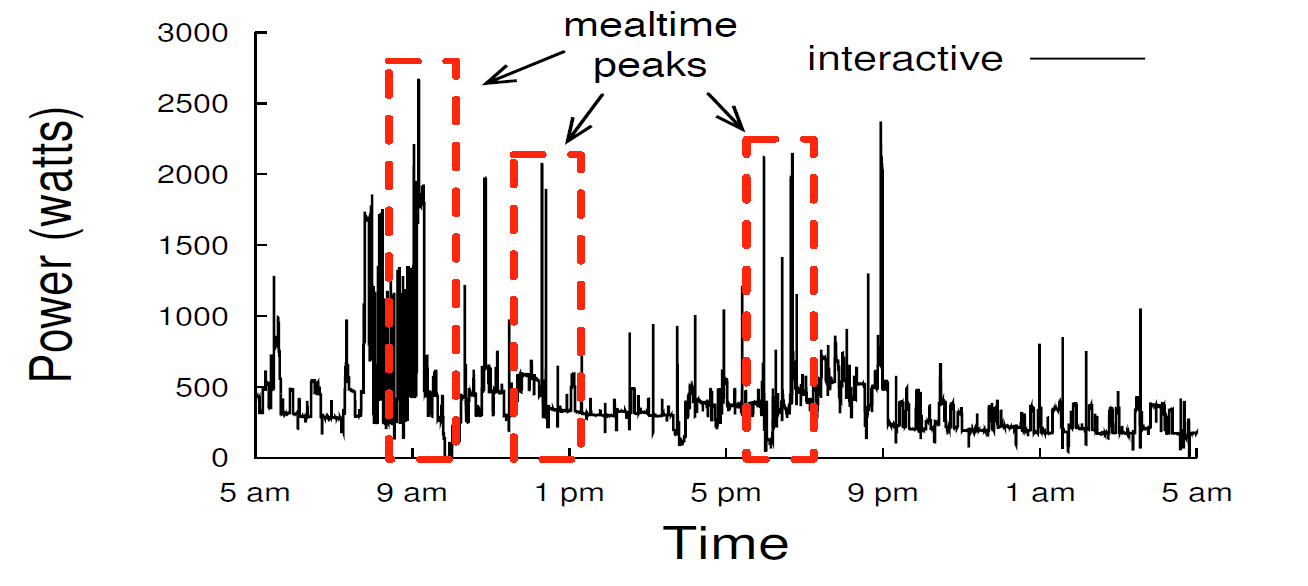
\includegraphics[width=1.0\textwidth]{img/peakdemand.png}
\caption[Peaks]{\emph{\small Power consumption in a household, meal time peaks highlighted \cite{barker2012smartcap}}}
\label{peakconsumption}
\end{figure}
 
We define two types of residential loads. The first one is referred to as background load. It consists of devices which are constantly plugged in, but does not always consume power, e.g. fridge, air condition and floor heating. The power units in these devices are only activated when the measured value from the environment(e.g. temperature) differs too much from the set value.

The second term is called the interactive load and consists of devices such as microwave, radio and TV. These devices are much harder to predict since people activate them when they need to use them. It is not possible to control the interactive load without interfering with the living habits of the residents. It should be pointed out that one goal of our work aims is to demonstrate a solution which do not disturb the residents of the house. We describe the solution in section \ref{sec:implementation}.

\subsection{Limitations}
The system is built in a small scale with limited test data to show the concept. The model will hold a couple of devices connected and monitored to test and validate the solution. We evaluate one of several possible solutions to the problem. Further solutions will be discussed in section \ref{sec:discussion}.

The data set we use for testing consists of 24 hours of data from a single household. We are aware of the limited test data and therefore we suggest that the algorithm should be tested more extensively by including more homes over a longer period to the test data.
%% Korrekturläst av Anders 2014-12-03
